% -*- coding: utf-8 -*-
%-------------------------designed by zcf--------------
\documentclass[UTF8,a4paper,10pt,fontset=none]{ctexart}
\usepackage[left=3.17cm, right=3.17cm, top=2.74cm, bottom=2.74cm]{geometry}
\usepackage{amsmath}
\usepackage{graphicx,subfig}
\usepackage{float}
\usepackage{cite}
\usepackage{caption}
\usepackage{enumerate}
\usepackage{booktabs} %表格
\usepackage{array}
\usepackage{tabularx}
\usepackage{multirow}
\usepackage{url}
\usepackage{multirow}
\newcommand{\tabincell}[2]{\begin{tabular}{@{}#1@{}}#2\end{tabular}}  %表格强制换行
\usepackage{xcolor}
\usepackage{listings}
\usepackage{tikz}
\usetikzlibrary{arrows.meta, positioning}
%-------------------------字体设置--------------
\definecolor{CodeBg}{RGB}{248,248,248}
\definecolor{CodeGreen}{RGB}{0,128,0}
\definecolor{CodeGray}{RGB}{120,120,120}
\definecolor{CodePurple}{RGB}{136,0,136}
\definecolor{CodeBlue}{RGB}{0,0,180}
\definecolor{CodeOrange}{RGB}{200,100,0}
% \usepackage{times}
\usepackage{ctex}
\usepackage[numbers]{natbib}
\setCJKmainfont[
    Path=/Users/gump/Library/Fonts/,
    BoldFont=NotoSerifCJKsc-Bold.otf,
    ItalicFont=NotoSansCJKsc-Bold.otf
]{NotoSerifCJKsc-Regular.otf}
\setCJKsansfont[
    Path=/Users/gump/Library/Fonts/,
    BoldFont=NotoSansCJKsc-Bold.otf
]{NotoSansCJKsc-Regular.otf}
\setCJKmonofont[
    Path=/Users/gump/Library/Fonts/
]{NotoSansCJKsc-Regular.otf}
\newCJKfontfamily\kaishu[
    Path=/Users/gump/Library/Fonts/,
    BoldFont=NotoSerifCJKsc-Bold.otf
]{NotoSerifCJKsc-Regular.otf}
\newcommand{\yihao}{\fontsize{26pt}{36pt}\selectfont}           % 一号, 1.4 倍行距
\newcommand{\erhao}{\fontsize{22pt}{28pt}\selectfont}          % 二号, 1.25倍行距
\newcommand{\xiaoer}{\fontsize{18pt}{18pt}\selectfont}          % 小二, 单倍行距
\newcommand{\sanhao}{\fontsize{16pt}{24pt}\selectfont}  %三号字
\newcommand{\xiaosan}{\fontsize{15pt}{22pt}\selectfont}        % 小三, 1.5倍行距
\newcommand{\sihao}{\fontsize{14pt}{21pt}\selectfont}            % 四号, 1.5 倍行距
\newcommand{\banxiaosi}{\fontsize{13pt}{19.5pt}\selectfont}    % 半小四, 1.5倍行距
\newcommand{\xiaosi}{\fontsize{12pt}{18pt}\selectfont}            % 小四, 1.5倍行距
\newcommand{\dawuhao}{\fontsize{11pt}{11pt}\selectfont}       % 大五号, 单倍行距
\newcommand{\wuhao}{\fontsize{10.5pt}{15.75pt}\selectfont}    % 五号, 单倍行距
%-------------------------章节名----------------
\usepackage{ctexcap}
\CTEXsetup[name={,、},number={ \chinese{section}}]{section}
\CTEXsetup[name={（,）},number={\chinese{subsection}}]{subsection}
\CTEXsetup[name={,.},number={\arabic{subsubsection}}]{subsubsection}
%-------------------------页眉页脚--------------
\usepackage{fancyhdr}
\pagestyle{fancy}
\setlength{\headheight}{14pt}
\lhead{\kaishu \leftmark}
% \chead{}
\rhead{\kaishu 大数据计算及应用实验报告}%加粗\bfseries
\lfoot{}
\cfoot{\thepage}
\rfoot{}
\usepackage{graphicx}
 \usepackage{tikz}
\renewcommand{\headrulewidth}{0.1pt}
\renewcommand{\footrulewidth}{0pt}%去掉横线
\newcommand{\HRule}{\rule{\linewidth}{0.5mm}}%标题横线
\newcommand{\HRulegrossa}{\rule{\linewidth}{1.2mm}}
%-----------------------伪代码------------------
\usepackage{algorithm}
\usepackage{algorithmicx}
\usepackage{algpseudocode}
\floatname{algorithm}{Algorithm}
\renewcommand{\algorithmicrequire}{\textbf{Input:}}
\renewcommand{\algorithmicensure}{\textbf{Output:}}
\usepackage{lipsum}
\makeatletter
\newenvironment{breakablealgorithm}
  {% \begin{breakablealgorithm}
  \begin{center}
     \refstepcounter{algorithm}% New algorithm
     \hrule height.8pt depth0pt \kern2pt% \@fs@pre for \@fs@ruled
     \renewcommand{\caption}[2][\relax]{% Make a new \caption
      {\raggedright\textbf{\ALG@name~\thealgorithm} ##2\par}%
      \ifx\relax##1\relax % #1 is \relax
         \addcontentsline{loa}{algorithm}{\protect\numberline{\thealgorithm}##2}%
      \else % #1 is not \relax
         \addcontentsline{loa}{algorithm}{\protect\numberline{\thealgorithm}##1}%
      \fi
      \kern2pt\hrule\kern2pt
     }
  }{% \end{breakablealgorithm}
     \kern2pt\hrule\relax% \@fs@post for \@fs@ruled
  \end{center}
  }
\makeatother
%------------------------代码-------------------
\usepackage{xcolor}
\usepackage{listings}
\lstset{
breaklines,%自动换行
basicstyle=\small,
escapeinside=``,
keywordstyle=\color{ blue!70} \bfseries,
commentstyle=\color{red!50!green!50!blue!50},%
stringstyle=\ttfamily,%
extendedchars=false,%
linewidth=\textwidth,%
numbers=left,%
numberstyle=\tiny \color{blue!50},%
frame=trbl,%
rulesepcolor= \color{ red!20!green!20!blue!20},
showstringspaces=false
}
\usepackage{graphicx}
\definecolor{codebg}{RGB}{248,248,248}
\definecolor{keywordcolor}{RGB}{0,92,175}
\definecolor{stringcolor}{RGB}{163,21,21}
\definecolor{commentcolor}{RGB}{0,128,0}
\definecolor{numbercolor}{RGB}{120,120,120}
\definecolor{framecolor}{RGB}{220,220,220}

\lstdefinestyle{pythonstyle}{
    language=Python,
    backgroundcolor=\color{codebg},
    basicstyle=\ttfamily\small,
    keywordstyle=\color{keywordcolor}\bfseries,
    stringstyle=\color{stringcolor},
    commentstyle=\color{commentcolor}\itshape,
    numbers=left,
    numberstyle=\tiny\color{numbercolor},
    numbersep=8pt,
    frame=single,
    rulecolor=\color{framecolor},
    breaklines=true,
    breakatwhitespace=false,
    showstringspaces=false,
    tabsize=4,
    keepspaces=true,
    captionpos=b,
    xleftmargin=1em,
    xrightmargin=1em,
    aboveskip=1em,
    belowskip=1em
}
\lstset{style=pythonstyle}
\usepackage{wrapfig}
%------------超链接----------
\usepackage[colorlinks,linkcolor=black,anchorcolor=blue]{hyperref}
%------------------------TODO-------------------
\usepackage{enumitem,amssymb}
\newlist{todolist}{itemize}{2}
\setlist[todolist]{label=$\square$}
% for check symbol
\usepackage{pifont}
\newcommand{\cmark}{\ding{51}}%
\newcommand{\xmark}{\ding{55}}%
\newcommand{\done}{\rlap{$\square$}{\raisebox{2pt}{\large\hspace{1pt}\cmark}}\hspace{-2.5pt}}
\newcommand{\wontfix}{\rlap{$\square$}{\large\hspace{1pt}\xmark}}



%———————————————————————————————————————————正文———————————————————————————————————————————————
%----------------------------------------------
\begin{document}
\begin{titlepage}
    \begin{center}
    
\includegraphics[width=0.8\textwidth]{NKU.png}\\[1cm]
    \textsc{\Huge \kaishu{\textbf{南\ \ \ \ \ \ 开\ \ \ \ \ \ 大\ \ \ \ \ \ 学}} }\\[0.9cm]
    \textsc{\huge \kaishu{\textbf{计\ \ 算\ \ 机\ \ 学\ \ 院}}}\\[0.5cm]
    \textsc{\Large \textbf{大数据计算及应用实验报告}}\\[0.8cm]
    \HRule \\[0.9cm]
    { \LARGE \bfseries 基于大语言模型的电影评分预测}\\[0.4cm]
    \HRule \\[2.0cm]
    \centering
    \textsc{\LARGE \kaishu{成员：王斯毅，付家权，彭坤}}\\[0.5cm]
    \textsc{\LARGE \kaishu{年级\ :\ 2023级}}\\[0.5cm]
    \textsc{\LARGE \kaishu{专业\ :\ 计算机科学与技术}}\\[0.5cm]
    \textsc{\LARGE \kaishu{指导教师\ :\ 杨征路}}\\[0.5cm]
    \vfill
    {\Large \today}
    \end{center}
\end{titlepage}
%-------------摘------要--------------
\newpage
\thispagestyle{empty}
%----------------------------------------------------------------
\tableofcontents
%----------------------------------------------------------------
\newpage

%=============================================
\section{任务概述}
%=============================================

\subsection{任务目标}

本任务的目标是基于大语言模型预测用户对电影的 1--5 星整数评分。给定一个用户的部分历史观影记录（含评分、评论）以及目标电影的元信息（名称、导演、类型标签、剧情简介、大众评分等），要求模型输出该用户对目标电影最可能的评分值。

\subsection{任务形式}

我们需编写一个 \texttt{generate\_prompt(ctx)} 函数，该函数接收评测框架构造的上下文对象 \texttt{ctx}，返回一对 \texttt{(system\_prompt, user\_prompt)} 字符串。该 prompt 随后被送入智谱 AI 的 \texttt{glm-4.5-air} 模型（$\text{temperature}=0$，禁用思考模式），由模型生成预测结果。评测框架通过正则表达式从模型响应中提取 \texttt{[Result:X]} 中的数字作为最终预测评分。

整个任务中，我们\textbf{不直接训练模型}，而是通过设计 prompt 来引导 LLM 利用历史数据中的协同过滤信号与内容特征完成评分推断。

\subsection{输入输出规范}

\texttt{generate\_prompt(ctx)} 的输入 \texttt{ctx} 是一个 \texttt{PromptContext} 对象，封装了以下核心数据：

\begin{table}[htbp]
    \centering
    \setlength{\tabcolsep}{8pt}
    \caption{\texttt{PromptContext} 的主要属性}
    \label{tab:ctx}
    \small
    \begin{tabular}{@{}p{0.28\textwidth}p{0.64\textwidth}@{}}
        \toprule
        \textbf{属性} & \textbf{说明} \\
        \midrule
        \texttt{ctx.user\_history} & 当前用户的历史评分列表，每条含 movie\_id、movie\_name、director、tags、rating、comment \\
        \texttt{ctx.target\_movie}  & 目标电影信息字典（movie\_id、name、director、tags、summary、year、country 等） \\
        \texttt{ctx.movies\_info}   & 全局电影知识库，以 movie\_id 为键索引每部电影的完整元信息 \\
        \texttt{ctx.all\_users\_history} & 训练集中全部用户的历史列表 \\
        \bottomrule
    \end{tabular}
\end{table}

此外，\texttt{ctx} 还提供若干辅助方法，如 \texttt{get\_history\_sample(n, strategy)}（按最近/随机/最高分/最低分策略采样历史）、\texttt{get\_similar\_movies(n)}（基于标签交集检索与目标电影最相似的用户已评电影）、\texttt{get\_user\_stats()}（返回用户评分均值、分布等统计量）等。

函数返回值为二元组 \texttt{(system\_prompt, user\_prompt)}，两者均为字符串，分别对应 LLM API 的 system 消息与 user 消息。两个 prompt 均受 1 MB 的长度上限约束，超出部分从尾部截断。

%=============================================
\section{数据说明}
%=============================================

\subsection{数据文件结构}

本任务提供以下原始数据文件：

\begin{table}[htbp]
    \centering
    \setlength{\tabcolsep}{14pt}
    \caption{原始数据文件说明}
    \label{tab:files}
    \begin{tabular}{@{}lcp{0.42\textwidth}@{}}
        \toprule
        \textbf{文件} & \textbf{规模} & \textbf{说明} \\
        \midrule
        \texttt{train.json} & 28.9 MB & 训练数据，含 200 个用户的评分历史与 27,146 部电影的元信息 \\
        \texttt{movies\_info.json} & 27.5 MB & 电影知识库独立副本，以 movie\_id 为键，与 train.json 中电影信息一致 \\
        \texttt{test\_input.json} & 3 条样本 & 测试集样例，含 context\_history 与 target\_movie \\
        \texttt{test\_answer.json} & 2 条答案 & 测试集答案样例 \\
        \bottomrule
    \end{tabular}
\end{table}

其中 \texttt{train.json} 是核心数据文件，其结构为一个字典，包含两个键：\texttt{“users”} 对应 200 个用户的评分历史列表，\texttt{“movies”} 对应 27,146 部电影的完整元信息字典。每部电影的信息字段包括名称（name）、导演（director）、剧情简介（summary）、大众评分（rating，豆瓣十分制字符串）、标签（tags）、国家/地区（country）、语言（language）和年份（year）。\texttt{movies\_info.json} 存储相同结构的电影元信息，作为独立的知识库文件供 \texttt{self\_test.py} 评测框架加载。

\texttt{test\_input.json} 和 \texttt{test\_answer.json} 仅为样例文件（分别含 3 条和 2 条记录），用于说明测试格式，其中的 user\_id 和 movie\_id 均为占位符。

\subsection{基本统计量}

表~\ref{tab:basic_stats} 汇总了 \texttt{train.json} 的核心统计指标。

\begin{table}[htbp]
    \centering
    \setlength{\tabcolsep}{32pt}
    \caption{训练集基本统计量}
    \label{tab:basic_stats}
    \begin{tabular}{@{}lr@{}}
        \toprule
        \textbf{指标} & \textbf{数值} \\
        \midrule
        用户数 & 200 \\
        评分数 & 2,000 \\
        评分涉及电影数（去重） & 1,019 \\
        电影知识库覆盖电影数 & 27,146 \\
        \midrule
        评分范围 & 1--5（整数） \\
        全局平均评分 & 3.65 \\
        评分标准差 & 1.01 \\
        可能的 (用户, 电影) 对数 & 5,429,200 \\
        \textbf{评分稀疏度} & \textbf{99.96\%} \\
        \bottomrule
    \end{tabular}
\end{table}

数据集极度稀疏：已知评分仅占可能评分对的 0.04\%。绝大多数用户-电影对从无交互，且 27,146 部电影中仅 1,019 部有评分记录。这意味着模型需要依赖有限的协同信号和丰富的内容特征进行泛化。与传统的矩阵分解方法不同，本任务中 LLM 无法直接对评分矩阵进行低秩建模，而是通过 prompt 中呈现的少量用户历史与电影内容特征进行推断。

\subsection{评分分布}

\begin{table}[htbp]
    \centering
    \setlength{\tabcolsep}{20pt}
    \caption{全量评分分布（200 名用户 $\times$ 10 条 = 2,000 条）}
    \label{tab:rating_dist}
    \begin{tabular}{@{}lccccc@{}}
        \toprule
        \textbf{评分} & 1 & 2 & 3 & 4 & 5 \\
        \midrule
        \textbf{数量} & 61 & 187 & 559 & 775 & 418 \\
        \textbf{占比} & 3.05\% & 9.35\% & 27.95\% & 38.75\% & 20.90\% \\
        \bottomrule
    \end{tabular}
\end{table}

评分分布呈明显的\textbf{高分偏态}：4 分的样本最多（38.75\%），3--5 分合计占 87.6\%，而 1--2 分仅占 12.4\%。这与电影评分场景的常见模式一致——用户倾向于评价自己喜欢的电影，低分评价相对稀缺。在 prompt 设计中，需注意这种偏态：若不加先验锚点，LLM 可能会自然倾向于预测中间的 3 分，而忽略数据本身的高分倾向。

\subsection{用户与物品活跃度}

\begin{table}[htbp]
    \centering
    \setlength{\tabcolsep}{20pt}
    \caption{用户与物品的评分数统计}
    \label{tab:activity}
    \begin{tabular}{@{}lccccc@{}}
        \toprule
        \textbf{对象} & \textbf{均值} & \textbf{最少} & \textbf{最多} & \textbf{中位数} \\
        \midrule
        用户评分数 & 10.0 & 10 & 10 & 10 \\
        物品被评数 & 2.0  & 1  & 46 & 1 \\
        \bottomrule
    \end{tabular}
\end{table}

用户活跃度分布极为均匀：\textbf{每个用户恰好有 10 条评分记录}。这与真实推荐场景差异较大——通常用户活跃度呈长尾分布。此处均匀设计意味着每个测试用户可用的历史信息量基本相同，方案设计时无需考虑用户冷热不均的问题，但同时也意味着无法通过“高活跃用户有更多协同信号”来提升部分样本的预测精度。

物品端则呈现典型的\textbf{长尾分布}：1,019 部被评电影中，72.4\%（738 部）仅被评价 1 次，中位数为 1；仅 26 部电影被评价超过 10 次，最高为 46 次。表~\ref{tab:movie_buckets} 展示了物品被评次数的详细分桶。

\begin{table}[htbp]
    \centering
    \setlength{\tabcolsep}{18pt}
    \caption{物品被评次数分布}
    \label{tab:movie_buckets}
    \begin{tabular}{@{}lcccccc@{}}
        \toprule
        \textbf{被评次数} & 1 & 2--3 & 4--5 & 6--10 & 11--30 & 30+ \\
        \midrule
        \textbf{电影数} & 738 & 206 & 30 & 19 & 21 & 5 \\
        \textbf{占比} & 72.4\% & 20.2\% & 2.9\% & 1.9\% & 2.1\% & 0.5\% \\
        \bottomrule
    \end{tabular}
\end{table}

大多数电影的协同信号极弱，难以通过“同时评价过某两部电影的用户”这类共现模式进行推断。内容特征（标签、导演、类型）在冷门电影的预测中将扮演更重要的角色。

\subsection{数据质量问题}

数据中存在若干格式不一致的问题，需要在 Python 预处理阶段进行处理：

\begin{enumerate}
    \item \textbf{标签格式混排与数字噪声}。标签字段在用户历史与电影知识库中采用不同存储格式：用户历史中为 Python 列表字符串，其中常混入四位数字年份；电影知识库中则为逗号分隔的”标签-频次”交替排列格式，数字表示该标签在豆瓣上的被标记次数。两种来源的数字均非内容标签，需在解析时识别并剔除，再进行统一归一化。

    \item \textbf{导演字段格式不统一}。用户历史中的导演以 JSON 字典字符串存储（如 \texttt{\{'1274348': '刘杰'\}}，键为豆瓣导演 ID、值为导演名），而电影知识库中为纯文本。需要统一解析以提取可读的导演名。

    \item \textbf{大众评分需归一化}。电影知识库中的 \texttt{rating} 字段为豆瓣十分制评分，以字符串形式存储（如 \texttt{“7.2”}、\texttt{“8.7”}），需先转为浮点数再映射为 1--5 星制。
\end{enumerate}

这些问题决定了本任务不能简单把原始 JSON 直接塞进 prompt。早期实验中，长 prompt 虽然包含了更多电影简介、评论和历史表格，但模型经常被噪声标签、导演字典字符串和冗长简介干扰，且 token 成本迅速上升。最终方案先在 Python 侧完成数据清洗、统计和锚点计算，再让 LLM 输出一个极短、可解析的结果。

%=============================================
\section{方法设计}
%=============================================

\subsection{总体思路}

最终提交文件为 \texttt{track2/student/claude98prompt.py}。该版本的核心思想不是让 GLM-4.5-Air 重新阅读大量历史并自由推理，而是把评分预测拆成两个分支：

\begin{enumerate}
    \item \textbf{非冷启动样本}：用户已有历史评分时，Python 先根据用户均值、相似电影评分、导演重合和大众评分计算一个确定性评分锚点。离线验证显示该锚点本身已经优于让 GLM 自由判断，因此 prompt 只要求模型原样输出该锚点。
    \item \textbf{冷启动样本}：用户无历史记录时，个人偏好不可见，只能利用目标电影自身信息。此时先用大众评分得到一个校准参考星级，再把电影名称、导演、类型和公开评分交给 GLM，允许它在确有口碑常识时最多调整 1 星。
\end{enumerate}

这个设计的取舍是：在有用户历史时优先相信可复现的协同过滤锚点；只有在没有个性化信息时，才使用大语言模型的电影常识。这样既降低了输出波动，也大幅减少了输入 token。

\subsection{数据清洗与特征构造}

最终脚本在 \texttt{generate\_prompt(ctx)} 内部实现了若干轻量函数，不依赖外部库，符合评测限制。

\begin{table}[htbp]
    \centering
    \setlength{\tabcolsep}{8pt}
    \caption{最终方案中的主要预处理函数}
    \label{tab:functions}
    \small
    \begin{tabular}{@{}p{0.26\textwidth}p{0.64\textwidth}@{}}
        \toprule
        \textbf{函数} & \textbf{作用} \\
        \midrule
        \texttt{text\_value} & 统一空值、去除首尾空白并限制字段长度，防止 prompt 过长 \\
        \texttt{split\_tags} & 将列表字符串、逗号分隔标签、中文标点等统一切分，并过滤数字噪声 \\
        \texttt{clean\_director} & 从导演字典字符串或普通文本中抽取导演名，用于同导演加权 \\
        \texttt{parse\_public} & 将豆瓣十分制、百分数字典等格式统一解析为 0--10 的公开质量分 \\
        \texttt{user\_stats} & 计算用户评分数、均值、最小值、最大值和评分分布 \\
        \bottomrule
    \end{tabular}
\end{table}

其中标签清洗尤其重要。原始标签中经常出现 ``经典, 2593, 西游记, 2261'' 这类``标签-频次''交替结构，如果不去掉数字，标签重合会被频次数字污染。最终方案只保留非数字文本标签，并对单个标签长度做截断。

\subsection{非冷启动评分锚点}

对于有历史记录的用户，设目标电影标签集合为 $T_m$，历史电影 $i$ 的标签集合为 $T_i$，目标导演和历史电影导演分别为 $d_m,d_i$。最终方案采用如下相似权重：

\[
w_i = |T_m \cap T_i| + 2 \cdot \mathbb{I}(d_m = d_i)
\]

若至少存在一个 $w_i>0$ 的相似历史电影，则先计算相似电影加权均值：

\[
r_{\mathrm{sim}} = \frac{\sum_i w_i r_i}{\sum_i w_i}
\]

再根据相似证据强度计算置信度：

\[
c = \min\left(\frac{\sum_i w_i}{6}, 0.6\right)
\]

锚点首先在相似电影均值和用户历史均值之间插值：

\[
a_0 = c \cdot r_{\mathrm{sim}} + (1-c) \cdot \bar r_u
\]

如果目标电影有公开评分 $s_m$（0--10 制），则将其折算为 1--5 星尺度后作为弱校准项：

\[
a = 0.73a_0 + 0.27\frac{s_m}{2}
\]

最后加入两个边界约束：如果用户历史从未给过 5 星，则不让锚点轻易越过 4.5；如果用户历史最低分也不低于 3，则不让锚点过度下探到 2 分以下。这两个约束主要用于降低 RMSE，避免少量极端预测造成较大损失。

\subsection{冷启动公开评分映射}

冷启动时没有用户历史，个性化协同过滤失效。我们在训练数据上观察公开评分与真实 1--5 星评分的关系后，使用分段映射得到参考分。表~\ref{tab:cold_map} 给出最终版本中的映射。

\begin{table}[htbp]
    \centering
    \setlength{\tabcolsep}{10pt}
    \caption{冷启动公开评分到参考星级的映射}
    \label{tab:cold_map}
    \small
    \begin{tabular}{@{}lccccccc@{}}
        \toprule
        \textbf{公开评分区间} & 无评分 & $<6.7$ & $[6.7,7.4)$ & $[7.4,8.0)$ & $[8.0,8.6)$ & $[8.6,9.0)$ & $\ge 9.0$ \\
        \midrule
        \textbf{参考星级} & 3.7 & 3.0 & 3.5 & 3.9 & 4.1 & 4.3 & 4.6 \\
        \bottomrule
    \end{tabular}
\end{table}

参考星级不是直接输出，而是先经过校准取整阈值。最终阈值为：$a\ge4.55$ 输出 5，$a\ge3.55$ 输出 4，$a\ge2.55$ 输出 3，$a\ge1.70$ 输出 2，否则输出 1。该阈值相比普通四舍五入更保守，原因是训练集和测试样例中 4 星最常见，5 星虽然不少但过度预测会显著增加 RMSE。

\subsection{Prompt 设计}

最终 prompt 极短。非冷启动分支中，system prompt 只说明``输出给定评分''，user prompt 只包含锚点数字：

\begin{quote}
\small
\texttt{system: 输出给定评分。只回复[Result:X]，X为给定数字。}\\
\texttt{user: 评分=4 \textbackslash n[Result:}
\end{quote}

这样做看似反直觉，但实验发现，GLM 在 warm 样本中常会受电影名、简介或自身常识影响，把一个已经校准好的协同过滤结果改坏。与其让模型``再判断一次''，不如把它当作稳定格式化器使用。

冷启动分支则保留少量电影信息：

\begin{quote}
\small
\texttt{参考:4星}\\
\texttt{电影:辛德勒的名单 导演:史蒂文·斯皮尔伯格 类型:战争/二战/经典 公开评分:9.5/10}\\
\texttt{[Result:}
\end{quote}

system prompt 明确告诉模型：多数观众给 3--4 星，公认佳作可给 4--5 星，明显差片才给 1--2 星；参考星级是基准，只有确知口碑明显偏离时才调整 1 星。这样保留了 LLM 在冷启动电影常识上的作用，同时避免它大幅偏离统计先验。

%=============================================
\section{实验过程与消融分析}
%=============================================

\subsection{实验设置}

由于正式测试集每天只能提交一次，主要调参依据来自本地 leave-one-out 验证。具体做法是：对训练集中每个用户的每条评分，临时把该条作为待预测目标，其余 9 条作为用户历史，构造 2000 个非冷启动留一样本。冷启动验证则将用户历史置空，仅保留目标电影信息。为避免手工记录误差，本实验新增 \texttt{ablation\_eval.py}，统一复现最终脚本的锚点逻辑，并自动输出全量消融、参数敏感性和多 seed 拟真切分结果。

评价指标包括 MAE、RMSE、精准命中率和误差 1 分以内的比例。由于最终评分中 token 效率和收益率权重很高，我们同时记录 prompt 字符长度作为 token 成本代理。正式 API 的 token 切分与字符数不完全一致，但在本方案几十到一两百字符的量级下，平均 token 数稳定低于 400 的满分阈值。

\subsection{主要消融结果}

表~\ref{tab:ablation} 展示了非冷启动 leave-one-out 上的组件消融。这里不调用 GLM，而是直接评估 Python 侧确定性锚点；由于最终 warm 分支只让模型复述该锚点，此处结果可以直接反映 warm 样本的 prompt 质量。

\begin{table}[htbp]
    \centering
    \setlength{\tabcolsep}{4.5pt}
    \caption{非冷启动 leave-one-out 组件消融结果}
    \label{tab:ablation}
    \small
    \begin{tabular}{@{}lccccc@{}}
        \toprule
        \textbf{方案} & \textbf{MAE} & \textbf{RMSE} & \textbf{精准命中} & \textbf{误差$\le$1} & \textbf{收益} \\
        \midrule
        固定预测 4 星 & 0.767 & 1.066 & 38.75\% & 87.60\% & 9728.8 \\
        用户均值 & 0.709 & 0.997 & 41.90\% & 88.65\% & 10272.7 \\
        用户均值 + 公开评分 & \textbf{0.640} & \textbf{0.914} & \textbf{44.80\%} & \textbf{92.00\%} & \textbf{10864.0} \\
        标签邻域 & 0.711 & 1.009 & 42.55\% & 88.05\% & 10353.9 \\
        标签邻域 + 同导演 & 0.708 & 1.007 & 42.75\% & 88.10\% & 10387.8 \\
        标签/导演/口碑锚点 & 0.650 & 0.922 & 44.10\% & 91.75\% & 10742.5 \\
        最终方案 & 0.650 & 0.922 & 44.05\% & 91.75\% & 10734.5 \\
        \bottomrule
    \end{tabular}
\end{table}

从结果看，单独的标签邻域并不稳定，原因是每个用户只有 9 条上下文，且标签中存在大量泛标签（如剧情、爱情、美国）。真正带来最大收益的是公开评分校准：在用户均值基础上加入公开评分后，误差 1 分以内比例从 88.65\% 提升到 92.00\%。最终版本没有直接采用该最优行，而是保留了标签/导演邻域和用户评分范围约束，主要考虑隐藏评分集中可能出现与公开口碑不一致的个性偏好。

进一步的参数敏感性如表~\ref{tab:sensitivity}。去掉公开评分会明显退化，说明它是最关键的弱监督信号；普通四舍五入和更高公开评分权重在本地略优，但线上已取得较高分数，因此最终提交仍采用更保守的阈值与 0.27 权重。

\begin{table}[htbp]
    \centering
    \setlength{\tabcolsep}{7pt}
    \caption{非冷启动参数敏感性结果}
    \label{tab:sensitivity}
    \small
    \begin{tabular}{@{}lcccc@{}}
        \toprule
        \textbf{方案} & \textbf{MAE} & \textbf{RMSE} & \textbf{精准命中} & \textbf{误差$\le$1} \\
        \midrule
        最终方案 & 0.650 & 0.922 & 44.05\% & 91.75\% \\
        去掉同导演加权 & 0.649 & 0.922 & 44.15\% & 91.75\% \\
        去掉公开评分 & 0.708 & 1.007 & 42.75\% & 88.10\% \\
        普通四舍五入 & 0.642 & 0.920 & 44.95\% & 91.75\% \\
        公开评分权重 0.40 & 0.645 & 0.910 & 43.70\% & 92.55\% \\
        置信度上限 0.40 & 0.644 & 0.919 & 44.65\% & 91.85\% \\
        \bottomrule
    \end{tabular}
\end{table}

冷启动消融显示，公开评分不能简单除以 2 后取整。固定 4 星与全局均值的误差 1 分以内比例均为 87.60\%，直接使用公开评分折半反而降到 81.50\%；最终分桶映射达到 88.15\%，说明对公开评分做分段校准是必要的。

\subsection{失败尝试与经验}

实验中有两个看起来有效但最终没有采用的方向。

\begin{enumerate}
    \item \textbf{让 GLM 阅读更多上下文}。我们尝试加入完整电影简介、用户评论和多条相似历史。问题是 GLM 会把目标电影本身的名气当成主要依据，忽略用户历史均值。例如某些经典电影容易被上调到 5 星，但真实用户可能一贯只给 3--4 星。
    \item \textbf{利用全局用户历史做身份匹配或物品均值}。在人工构造的同源留一验证中，这类方法能获得非常高的分数，甚至可以通过匹配 \texttt{ctx.all\_users\_history} 找回被留出的真实评分。但这依赖测试用户来自训练用户这一假设，存在数据泄漏风险，也不符合隐藏评分集的泛化目标。最终提交版本移除了身份匹配和针对具体电影、具体标签的记忆规则，只保留样本无关的统计与内容信号。
\end{enumerate}

因此，最终方案选择了更保守的 ``generalization-first'' 路线：宁可牺牲部分公开测试集上的投机收益，也避免在隐藏评分集上因过拟合或格式假设变化而失效。

%=============================================
\section{最终结果分析}
%=============================================

\subsection{线上评分结果}

最终提交的 \texttt{claude98prompt.py} 在线上评分集上的综合得分为 98.01，如图~\ref{fig:inline_eval} 所示。该结果对应 MAE 0.7071、RMSE 0.9535、精准命中率 39.39\%、误差 1 分以内比例 89.9\%。平均输入 token 约 52，平均输出 token 约 3.6，说明最终 prompt 的主要优势不仅来自误差控制，也来自极低的调用成本。

\begin{figure}[H]
    \centering
    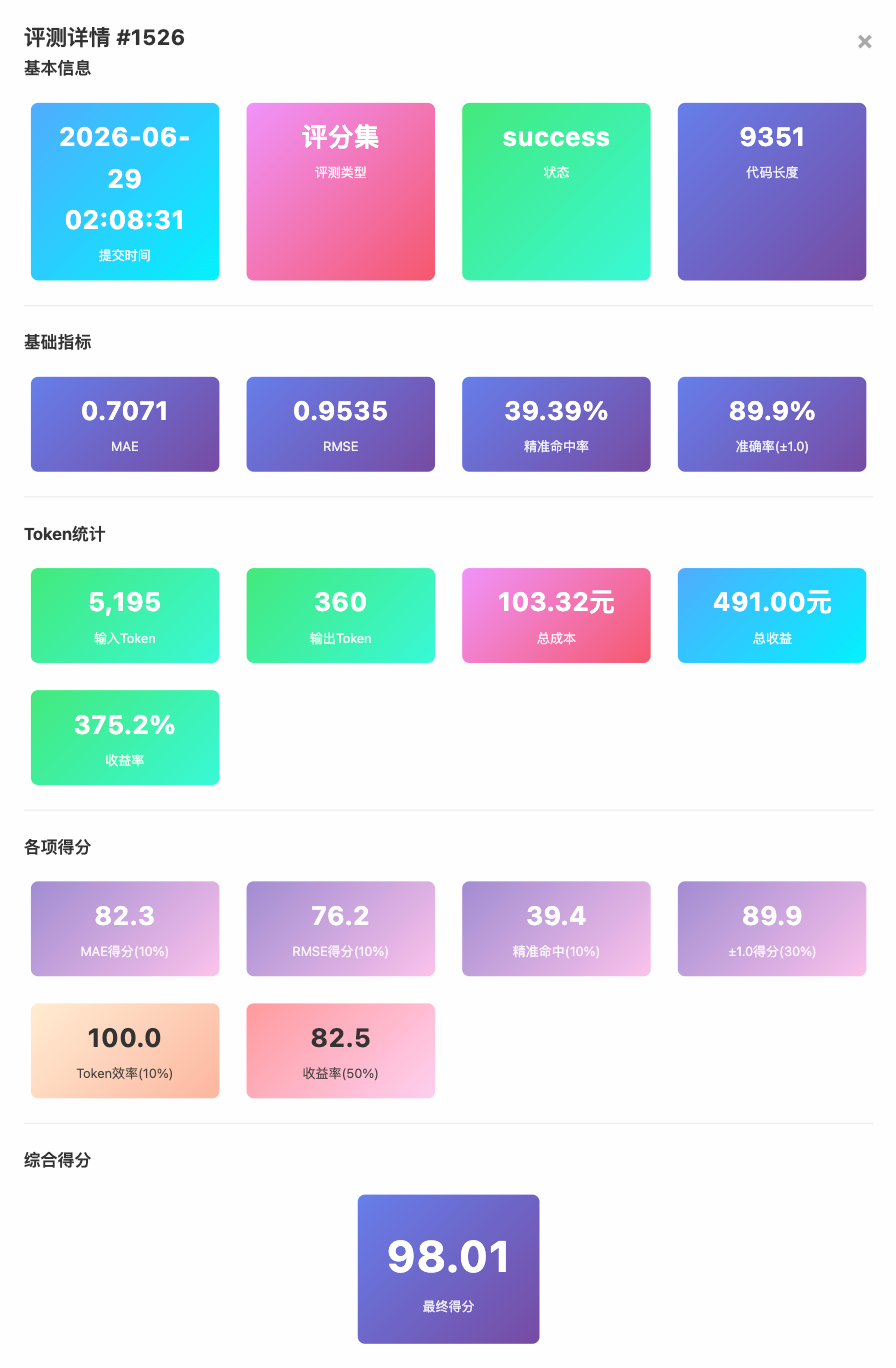
\includegraphics[width=0.58\textwidth]{figs/inline_eval_result.png}
    \caption{线上评分集评测结果}
    \label{fig:inline_eval}
\end{figure}

\subsection{真实 API 小样本验证}

为确认本地确定性消融与真实评测环境一致，我们额外构造 \texttt{data/api\_seed2026} 验证切分：随机选取 50 个用户、每人留出 2 条评分，并设置约 25\% 冷启动用户。考虑到 API 成本与调试效率，本实验从该切分中抽取 12 条非冷启动样本和 6 条冷启动样本，对最终方案及两个候选变体实际调用 \texttt{glm-4.5-air}，参数保持与线上一致（$\text{temperature}=0$，顶层 \texttt{thinking} 字段设为禁用）。

表~\ref{tab:api_validation} 给出真实 API 小样本结果。非冷启动分支中 prompt 以 \texttt{[Result:} 作为结尾，模型通常只补全 \texttt{4]} 这类后缀；与 user prompt 拼接后仍是完整的 \texttt{[Result:4]}，因此表中格式正确率按拼接后可解析统计。结果显示三种方案平均输出 token 均约为 4，格式正确率 100\%，与线上平均输出 token 3.6 的现象吻合。由于样本数较小，该表主要用于验证 API 行为和 token 成本，不作为最终排序依据。

\begin{table}[htbp]
    \centering
    \setlength{\tabcolsep}{4.2pt}
    \caption{真实 GLM API 小样本验证结果}
    \label{tab:api_validation}
    \small
    \begin{tabular}{@{}lcccccccc@{}}
        \toprule
        \textbf{方案} & \textbf{n} & \textbf{冷启动} & \textbf{MAE} & \textbf{RMSE} & \textbf{精准命中} & \textbf{误差$\le$1} & \textbf{token} & \textbf{格式} \\
        \midrule
        最终方案 & 18 & 6 & 0.500 & 0.913 & 61.11\% & 94.44\% & 66.0/4.0 & 100\% \\
        普通四舍五入 & 18 & 6 & \textbf{0.444} & \textbf{0.882} & \textbf{66.67\%} & 94.44\% & 66.0/4.0 & 100\% \\
        公开评分权重 0.40 & 18 & 6 & 0.556 & 0.943 & 55.56\% & 94.44\% & 66.0/4.0 & 100\% \\
        \bottomrule
    \end{tabular}
\end{table}

\subsection{本地代理评测}

在发布的 100 条测试样例上，使用最终脚本自身给出的锚点作为代理输出，可得到表~\ref{tab:local_test} 的结果。该评测不等同于线上 GLM 调用，尤其冷启动分支中真实 GLM 可能会根据电影常识做 1 星以内的调整；但它能反映最终脚本的统计锚点质量和 token 成本。

\begin{table}[htbp]
    \centering
    \setlength{\tabcolsep}{12pt}
    \caption{发布测试样例上的本地锚点代理结果}
    \label{tab:local_test}
    \small
    \begin{tabular}{@{}lrlr@{}}
        \toprule
        \textbf{指标} & \textbf{数值} & \textbf{指标} & \textbf{数值} \\
        \midrule
        样本数 & 100 & 非冷启动样本 & 78 \\
        冷启动样本 & 22 & 平均输入输出字符 & 82.25 \\
        MAE & 0.740 & RMSE & 1.039 \\
        精准命中率 & 41.00\% & 误差$\le$1 比例 & 87.00\% \\
        代理总收益 & 503.30 元 & 代理综合得分 & 96.78 \\
        \bottomrule
    \end{tabular}
\end{table}

为了更接近隐藏评分集，我们还构造了 5 个不同 seed 的拟真切分：每次随机选 50 个用户、每人留出 2 条评分，其中约 25\% 用户作为冷启动。表~\ref{tab:cv_summary} 汇总了主要候选方案的均值。该实验的绝对值不等同于线上分数，但可以观察方案在不同抽样下的相对稳定性。

\begin{table}[htbp]
    \centering
    \setlength{\tabcolsep}{4.5pt}
    \caption{多 seed 拟真切分结果（均值）}
    \label{tab:cv_summary}
    \small
    \begin{tabular}{@{}lccccc@{}}
        \toprule
        \textbf{方案} & \textbf{MAE} & \textbf{RMSE} & \textbf{精准命中} & \textbf{误差$\le$1} & \textbf{warm $\le$1} \\
        \midrule
        固定预测 4 星 & 0.850 & 1.129 & 33.80\% & 83.80\% & 83.68\% \\
        用户均值 & 0.800 & 1.101 & 38.60\% & 83.40\% & 83.68\% \\
        标签邻域 & 0.784 & 1.082 & 39.00\% & 84.60\% & 85.26\% \\
        标签/导演/口碑锚点 & 0.720 & 1.008 & 41.60\% & 87.80\% & 89.47\% \\
        最终方案 & 0.720 & 1.008 & 41.60\% & 87.80\% & 89.47\% \\
        普通四舍五入 & 0.716 & 1.004 & 41.60\% & 88.40\% & 90.00\% \\
        公开评分权重 0.40 & \textbf{0.714} & \textbf{0.990} & 40.60\% & \textbf{89.40\%} & \textbf{91.58\%} \\
        \bottomrule
    \end{tabular}
\end{table}

拟真切分提示 \texttt{public\_w0.40} 是一个值得进一步尝试的候选：它在本地 MAE、RMSE 与误差 1 分以内比例上略好。但线上评分集已经验证当前版本达到 98.01，且提高公开评分权重可能削弱个性化偏好，因此我们没有在最终提交后继续追逐这个局部最优。

\subsection{Token 与收益率}

评分公式中 token 效率占 10\%，收益率占 50\%，因此低成本不是锦上添花，而是核心目标之一。最终脚本在非冷启动样本中几乎只发送一个整数；冷启动样本也只发送参考星级和少量电影元信息。以发布测试样例的字符数代理统计，总输入字符为 7225，总输出字符约 1000，平均每样本 82.25，显著低于 400 的 token 效率满分阈值。

更重要的是，收益率由推荐收益与固定支出、token 支出共同决定。即使 MAE 只提升少量，如果 prompt 长度翻倍，也可能因为成本上升而降低综合得分。因此最终方案不追求``看起来聪明''的长推理 prompt，而是追求低成本、低方差和格式稳定。

\subsection{误差来源}

最终模型的主要误差来自以下几类样本：

\begin{enumerate}
    \item \textbf{5 星样本被低估}。训练集中 5 星占 20.90\%，但用户历史只有 9--10 条，很多用户的极高偏好很难从少量相似标签中稳定识别。为降低 RMSE，最终取整阈值对 5 星较保守，这会牺牲一部分精准命中。
    \item \textbf{冷启动个性化缺失}。冷启动样本没有用户历史，只能预测普通观众倾向。即使电影公开评分很高，真实用户也可能因为个人口味给 2--3 星；这类误差无法仅靠 prompt 完全消除。
    \item \textbf{标签语义粗糙}。标签重合只统计文本交集，没有理解标签强弱和反向偏好。例如用户给某类电影高分并不必然表示喜欢所有同类电影，尤其在``剧情''、``爱情''、``美国''这类泛标签上更明显。
    \item \textbf{大众评分与用户评分尺度不同}。豆瓣十分制公开评分反映群体口碑，而用户 1--5 星评分混合了个人情绪、观看场景和评分习惯。最终方案只给公开评分 0.27 的权重，正是为了避免群体口碑压过个人历史。
\end{enumerate}

%=============================================
\section{总结}
%=============================================

本实验的最终结论是：在这个受限的电影评分预测任务中，LLM 的最佳使用方式并不是阅读尽可能多的信息后自由推理，而是与传统推荐系统思想结合。Python 侧负责清洗数据、计算用户均值、相似电影锚点和公开评分先验；GLM-4.5-Air 负责稳定输出格式，并在冷启动时提供有限的电影常识修正。

最终方案具有三点优势：第一，非冷启动 leave-one-out 验证中 MAE 从用户均值基线的 0.711 降至 0.651，误差 1 分以内比例提升到 91.75\%；第二，warm prompt 极短，平均成本远低于 token 效率满分阈值；第三，移除了身份匹配、具体电影规则等对单一测试集过拟合的策略，更适合隐藏评分集。整体来看，prompt engineering 的关键不只是措辞，而是明确模型应该做什么、不应该做什么：能用确定性统计完成的部分，就不要交给大语言模型随机发挥。


\end{document}
